\chapter{Vymezení pojmů - 5 stran}

V této kapitole se budeme zabývat zejména dvěma pojmy. Těmito pojmy jsou IEQ (Indoor Environment Quality) a IAQ (Indoor Air Quality).
\section{IAQ a IEQ}
\subsection{IAQ}
Začneme pojmem IAQ, který je podmnožinou pojmu IEQ (obr. \ref{obr01:vztah_ieq_a_iaq}).

\begin{figure}[h]
	\centerfirst
	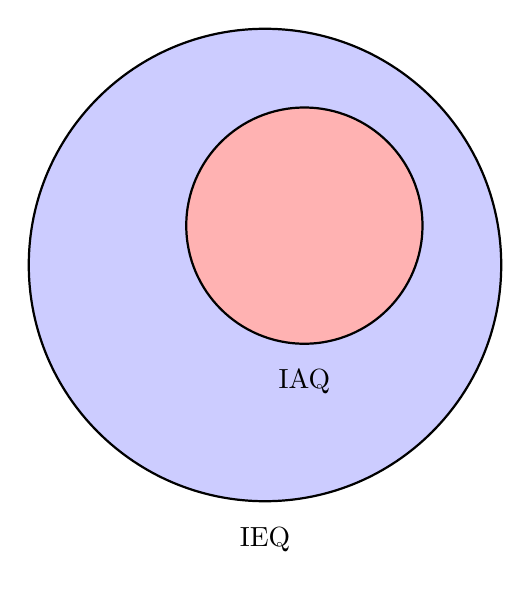
\begin{tikzpicture}
		% Množina IEQ
		\draw[thick, fill=blue!20] (0,0) circle (3cm) node[below] at (0,-3.2) {IEQ};
		
		% Množina IAQ
		\draw[thick, fill=red!30] (0.5,0.5) circle (1.5cm) node[below] at (0.5,-1.2) {IAQ};
	\end{tikzpicture}
	\caption{Vztah mezi IEQ a IAQ}
	\label{obr01:vztah_ieq_a_iaq}
\end{figure}

Pojem IAQ je zkratkou pro vnitřní kvalitu ovzduší. Tento je souborem mnoha veličin, které se týkají ovzduší. Mnohé z obsažených veličin jsou shodné s těmi pro vnější prostředí.
WHO (World Health Organization) vymezuje kvalitu ovzduší pomocí úrovní znečisťujících látek PM\textsubscript{2.5}\footnote{Particulate Matter $2.5\,\mu\text{m}$}, PM\textsubscript{10}\footnote{Particulate Matter $10\,\mu\text{m}$}, O\textsubscript{3} (Ozón), NO\textsubscript{2} (Oxid dusičitý), SO\textsubscript{2} (Oxid siřičitý) a CO (Oxid uhelnatý) . Všechny zmíněné veličiny jsou znečisťující látky, které mají negativní vliv na člověka \parencite{worldhealthorganizationWHOGlobalAir2021}.

Látky PM\textsubscript{2.5} a PM\textsubscript{10} jsou částicemi v ovzduší, které mají stejné aerodynamické vlastnosti jako jednolitá koule o průměrech 2,5 a 10 $\mu\text{m}$. Tyto částice se mohou dostat do plic člověka a v některých případech i do krevního řečiště. Mohou způsobovat astma, istemickou chorobu srdeční, srdeční selhání nebo chronickou obstrukční plicní nemoc \parencite{usepaIndoorPollutantsSources2015}. Na webu Úřadu pro ochranu životního prostředí USA\footnote{www.epa.gov} lze najít další znečisťující látky jako radon, VOC (Volatile Organic Compounds), plíseň, bakterie, viry, pesticidy, cigaretový kouř a aerosoly a další. Za zmínku stojí zejména VOC a radon.  VOC jsou plyny, které se uvolňují z některých pevných či kapalných látek. Mohou způsobovat podráždění nosy a očí, bolest hlavy a nevolnost, poškození jater, ledvin a CNS (centrální nervová soustava) a rakovinu \parencite{usepaIndoorPollutantsSources2015}.
Nesmíme zapomenout na CO\textsubscript{2}, které při vysokých koncentracích přispívá k zhoršeným kognitivním schopnostem a stresu\parencite{dengImpactIndoorAir2024}.

\subsection{IEQ}
Jak již bylo řečeno, IAQ je podmnožinou IEQ. Definice IEQ se dá rozšířit o tři kategorie. Těmi jsou \textit{tepelný komfort}, \textit{vizuální kompfort} a \textit{akustický komfort}. Tyto kategorie společně s IAQ tvoří prostředí, ve kterém se člověk pohybuje. Součástí tepelného komfortu je pak vlhkost, teplota vzduchu, teplota povrchu, rychlost vzduchu, míra aktivity člověka, oblečení \parencite{dengImpactIndoorAir2024}.

Vizuální komfort se skládá z vizálné ergonomiky, oslnění, přírodního osvětlení, umělého osvětlení, výhledu, soukromí a designem budovy\parencite{dengImpactIndoorAir2024}.

Akustický komfort se skládá z odhlučnění, míry hluku a soukromí\parencite{dengImpactIndoorAir2024}.

Je důležité si všimnout, že ne všechny veličiny, které IEQ nově přináší jsou dobře měřitelné. Zejména veličiny jako oblečení, vizuální komfort, soukromí, výhled a design budovy jsou velice těžko měřitelné a často subjektivní. Přesto nesmíme zapomínat, že nějakou váhu mají.

\subsection{Standardy}

V ČR se úrovně znečištění ovzduší řídí podl\textit{e zákona 201/2012 Sb. o ochraně ovzduší úplné a aktualní znění}. Ten ve své první příloze stanovuje imisní limity pro ochranu zdraví a maximální počet překročení těchto limitů \parencite{wolterskluwerZakon20120122012}. Limity převzané z tabulky v zákoně lze vidět v tabulce \ref{tab:imisni_limity_zdravi_cr}.


\begin{table}[h]
	\centering
	\caption{Imisní limity}
	\label{tab:imisni_limity_zdravi_cr}
	\begin{tabular}{|c|c|c|c|}
			\toprule 
			\textbf{Znečisťující látka} & \textbf{Doba průměrování}  & \textbf{Imisní limit}  & \textbf{Max. počet překročení} \\
			\midrule
			 SO\textsubscript{2} & 1 h & $350\, \mu\text{g}*m^{-3}$ & 24\\
			 SO\textsubscript{2} & 24 h &  $125\, \mu\text{g}*m^{-3}$ & 3\\
			 NO\textsubscript{2}&1 h &  $200\, \mu\text{g}*m^{-3} $ &  18\\
			 NO\textsubscript{2}&1 rok &  $40\, \mu\text{g}*m^{-3} $ &  0\\
			 CO& max. denní 8 h průměr &  $10\, \mu\text{g}*m^{-3} $ &  0\\
			 PM\textsubscript{10}&24 h &  $50\, \mu\text{g}*m^{-3} $ &  35\\
			 PM\textsubscript{10}&1 rok &  $40\, \mu\text{g}*m^{-3} $ &  0\\
			 PM\textsubscript{2.5}&1 rok &  $20\, \mu\text{g}*m^{-3} $ &  0\\
			 \bottomrule
		\end{tabular}
\end{table}

Také existuje směrnice WHO, která udává doporučení pro tyto látky. Tato směrnice se nazývá AQG (Air Quality Guidelines). Doporučení plynoucí z této směrnice naleznete v tabulce \ref{tab:doporucene_vystaveni_who} \parencite{worldhealthorganizationWHOGlobalAir2021}.

\begin{table}[h]
	\centering
	\caption{Doporučené úrovně vystavení dle WHO}
	\label{tab:doporucene_vystaveni_who}
	\begin{tabular}{|c|c|c|}
		\toprule 
		\textbf{Znečisťující látka} & \textbf{Doba průměrování}  & \textbf{úroveň AQG}  \\
		\midrule
		SO\textsubscript{2} & 24 h &  $40\, \mu\text{g}*m^{-3}$ \\
		NO\textsubscript{2}&24 h &  $25\, \mu\text{g}*m^{-3} $  \\
		NO\textsubscript{2}&1 rok &  $10\, \mu\text{g}*m^{-3} $  \\
		CO & 24 h &  $4\, \text{mg}*m^{-3} $ \\ 
		PM\textsubscript{10}&24 h &  $45\, \mu\text{g}*m^{-3} $ \\
		PM\textsubscript{10}&1 rok &  $15\, \mu\text{g}*m^{-3} $ \\
		PM\textsubscript{2.5}&24 h &  $15\, \mu\text{g}*m^{-3} $ \\
		PM\textsubscript{2.5}&1 rok &  $5\, \mu\text{g}*m^{-3} $ \\
		\bottomrule
	\end{tabular}
\end{table}

Pro CO\textsubscript{2} jsou limity stanoveny na $9000\,mg*m^{-3}$ (4921 ppm) během pracovní doby osmi hodin. Pro dobu kratší cca 15 min je tato koncentrace pak $45000\,mg*m^{-3}$ (24603 ppm) \parencite{wolterskluwerNarizeni36120072007}.

\section{Open data}


%Z těchto zdorojů bylo zjištěno, že IEQ se skládá z v podstatě ze čtyř částí. Těmi jsou IAQ, tepelný komfort, vizuální komfort a akustický komfort \parencite{dengImpactIndoorAir2024}. Detail toho, z čeho se tyto části skládají je uveden v tabulce \ref{tab:detail-casti-ieq}.

%\begin{table}[h]
%	\centering
%	\caption{Detail částí IEQ}
%	\label{tab:detail-casti-ieq}
%	\begin{tabular}{|c|c|c|c|}
%		\toprule 
%		\textbf{IAQ} & \textbf{tepelný komfort}  & \textbf{vizuální komfort}  & \textbf{akustický komfort} \\
%		\midrule
%		PM\textsubscript{2.5} & Rychlost vzduchu  	&  Vizuální komfort  & Zvuková izolace \\
%		PM\textsubscript{10}  & Vlhkost  					& Vizuální ergonomika  & Míra hluku \\
%		Ozone							 & Teplota vzduchu  	& Záře  & kkt \\
%		CO\textsubscript{2}	   & Teplota povrchů  		& Přírodní osvětlení  & Soukromí \\
%		SO\textsubscript{2}    & Míra aktivity 				 &  Umělé osvětlení &  \\
%		CO 								    & Oblečení/Izolace  	& Výhled  &  \\
%		Zápach 							&   								& Soukromí  &  \\
%		Míra větrání 				 &   									& Design budovy  &  \\
%		\bottomrule
%		
%	\end{tabular}
%\end{table}

